\documentclass{article}
%==============================================================================%
%	                          Packages                                     %
%==============================================================================%
% Packages
\usepackage[utf8]{inputenc}
\usepackage{graphicx}
\usepackage{amsmath}
\usepackage{amssymb}
\usepackage{braket}
\usepackage[margin=0.7in]{geometry}
\usepackage[version=4]{mhchem}
\usepackage{float}
%==============================================================================%
%                           User-Defined Commands                              %
%==============================================================================%
% User-Defined Commands
\newcommand{\be}{\begin{equation}}
\newcommand{\ee}{\end{equation}}
\newcommand{\benum}{\begin{enumerate}}
\newcommand{\eenum}{\end{enumerate}}
\newcommand{\pd}{\partial}
\newcommand{\dg}{\dagger}
%==============================================================================%
%                             Title Information                                %
%==============================================================================%
\title{Chem237: Lecture 7}
\date{4/17/18}
\author{Shane Flynn}
%==============================================================================%
\begin{document}
\maketitle

\section*{More Complex Calculus}
Consider
\be
I = \int_0^\infty dx \quad \frac{1}{1+x^3}
\ee
We know that we want to use the residue to compute this integral, so we need to find the poles (which means we need the roots of the associated complex equation). 
\be
\begin{split}
    1 + z^n &= 0 \Rightarrow z^n - 1 = 0\\
    |z|^n = |1|
\end{split}
\ee
So we need exactly n roots (root sof unity), consider the unit circle 

\begin{figure}[H]
  \centering
    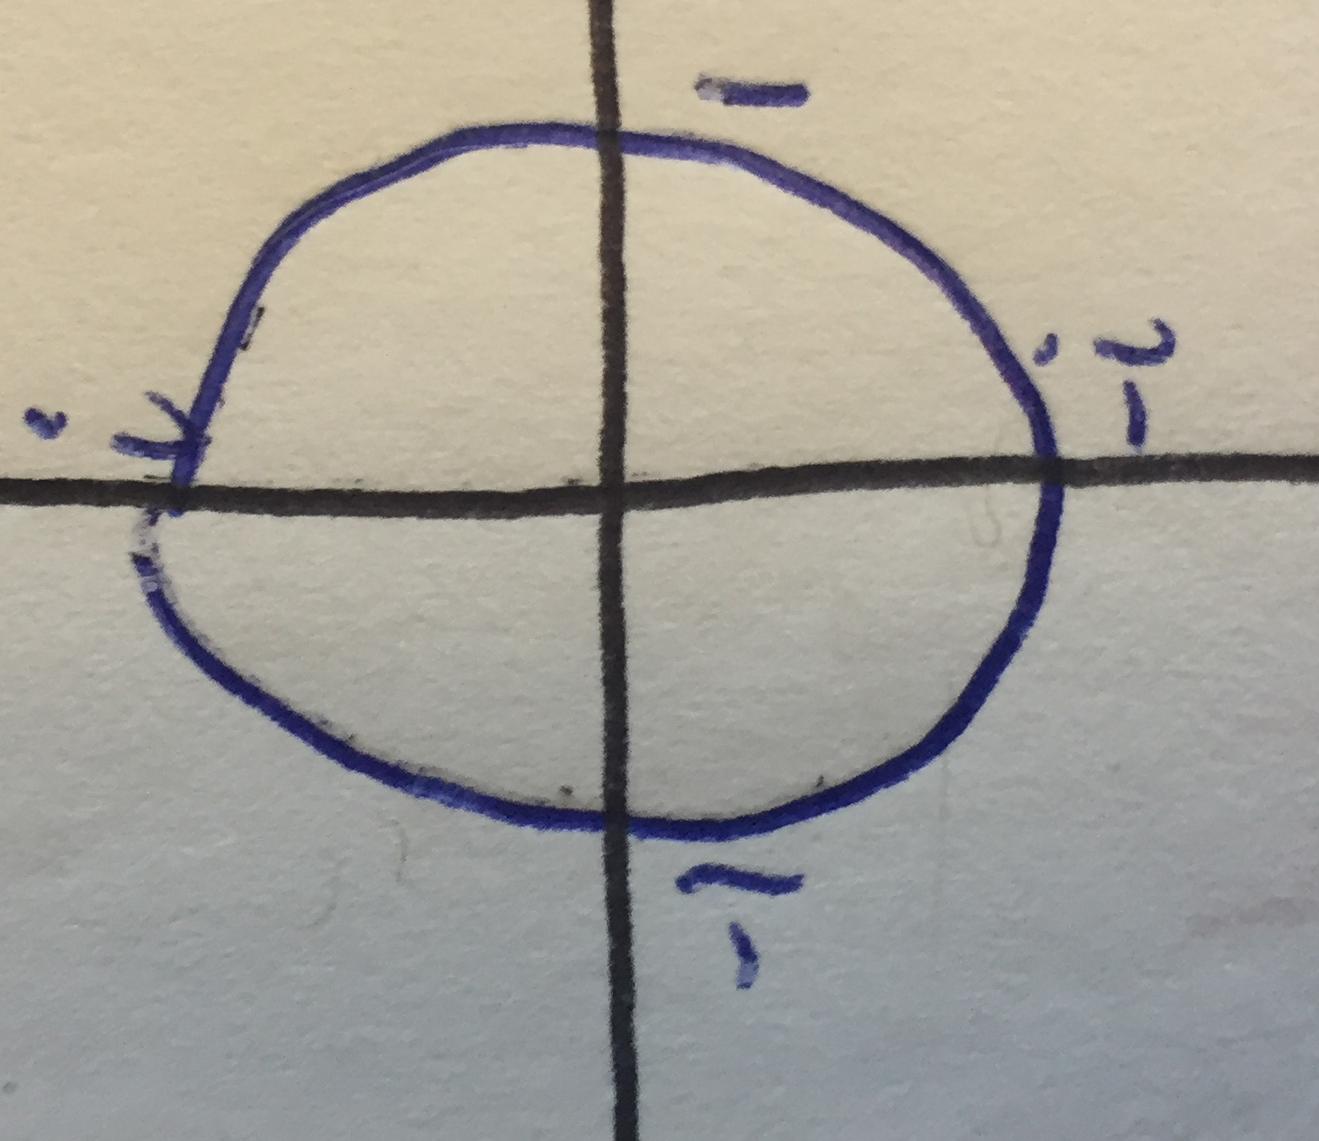
\includegraphics[scale=0.2]{Figures/unit.png}
    \caption{Make a caption. Unit Circle for real/complex}
\end{figure}

All of the roots must be on the unit circle, we can define a complex number z as $z=e^{i\theta}$, which will be on the unit circle. 
\be
1 = e^{ian}, \quad \theta = \frac{2\pi k}{n} \Rightarrow 1 = e^{2\pi ik}
\ee
Where k runs from 0,1,2,3,...,n-1 (to give a total of n roots). 

So we can now find the roots
\be
1+z^n \Rightarrow e^{i\theta n} = 1 - e^{i2\pi k + i\pi} \rightarrow \theta = \frac{2\pi k}{n} + \frac{\pi}{n}
\ee

Returning to our example we can find the first 3 roots for 1 + $|x|^3$ as:  $e^{\frac{i2\pi}{6}}, e^{\frac{-i2\pi}{6}}, -1 $.
So we have foudn our 3 poles for this system. 
\begin{figure}[H]
  \centering
    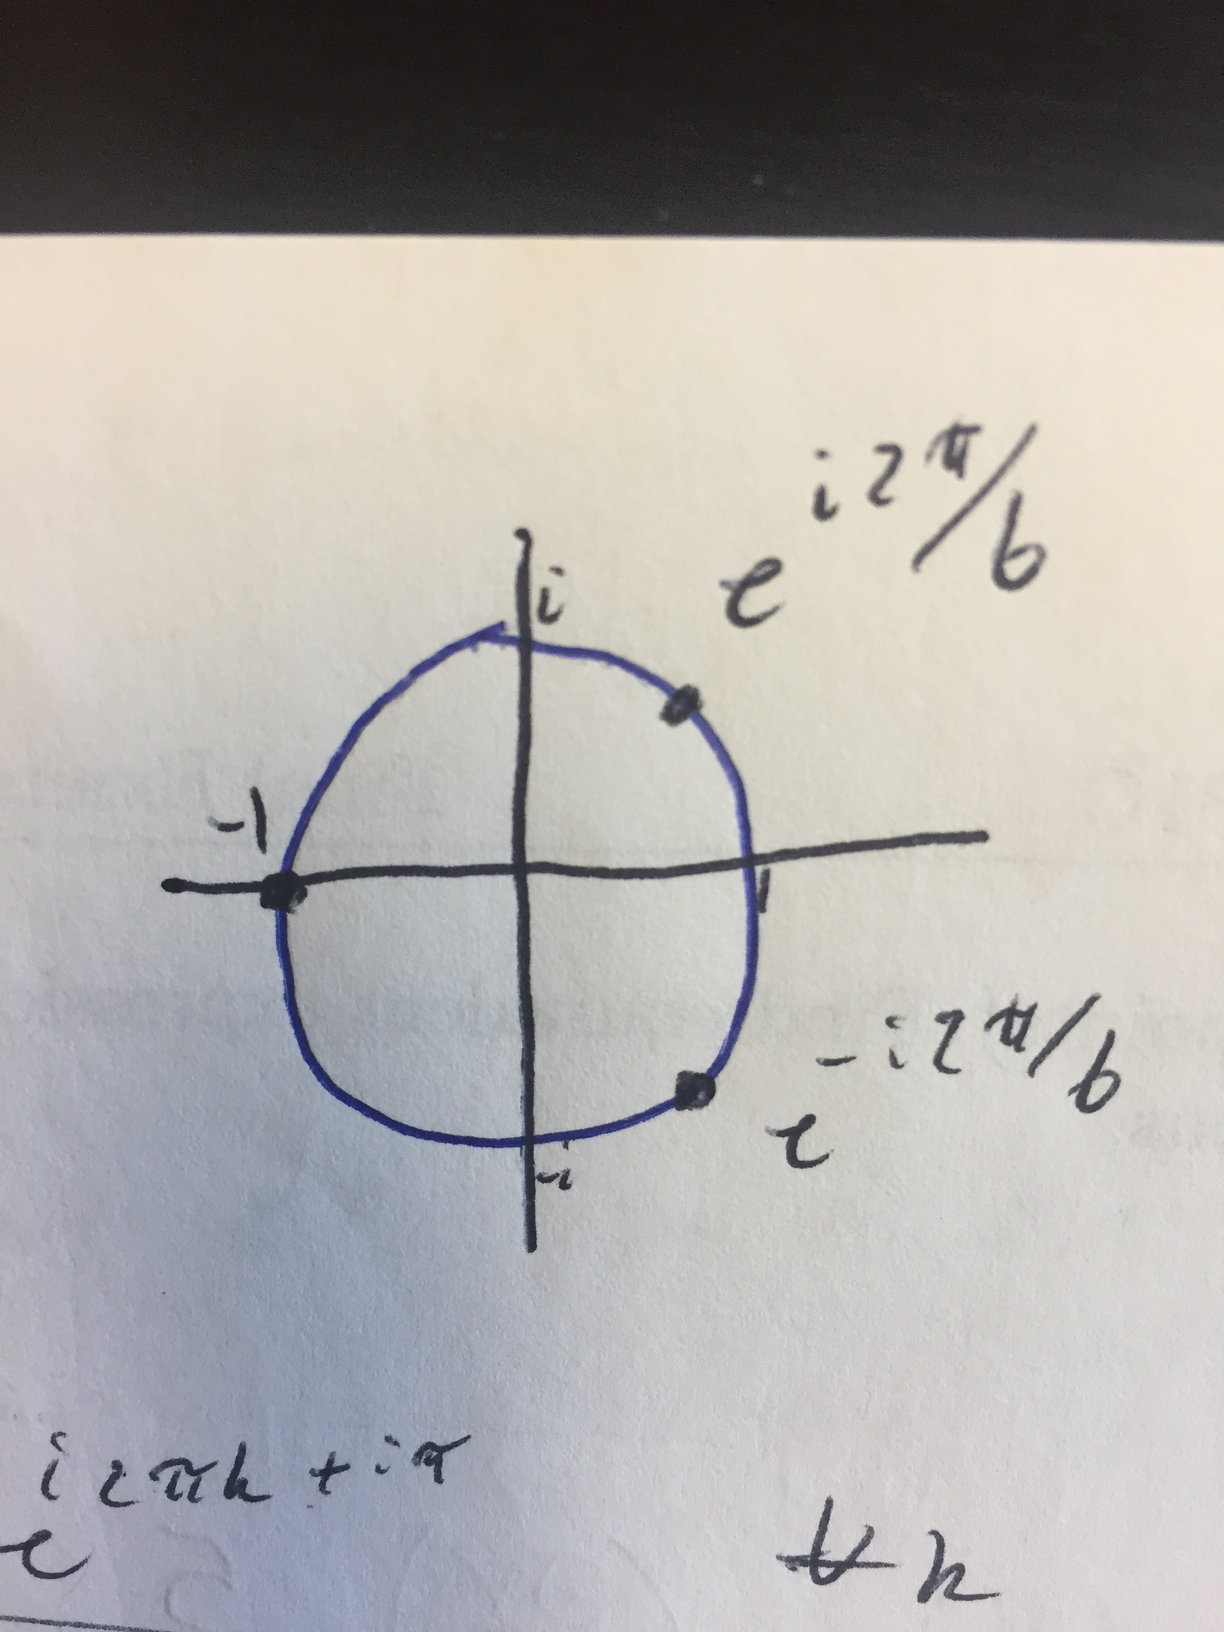
\includegraphics[scale=0.2]{Figures/poles.png}
    \caption{Make a caption. 3 Poles for Cubic Equation}
\end{figure}

But we have a problem now, our integral bounds go from 0 to infinity, our function is not even so we cannot simply change the bounds.

There are two ways we can continue, both will require those poles we just found. 

This first trick is to actually consider a different problem, consider
\be
\oint dz \quad \frac{\ln|z|}{1+z^3}
\ee

Why we are considering this other problem is not clear right now, but we will see.
Unfortunatley the natural logarithm has a branching point, but we can get around this problem (at 0) with an interesting looking contour. 
\begin{figure}[H]
  \centering
    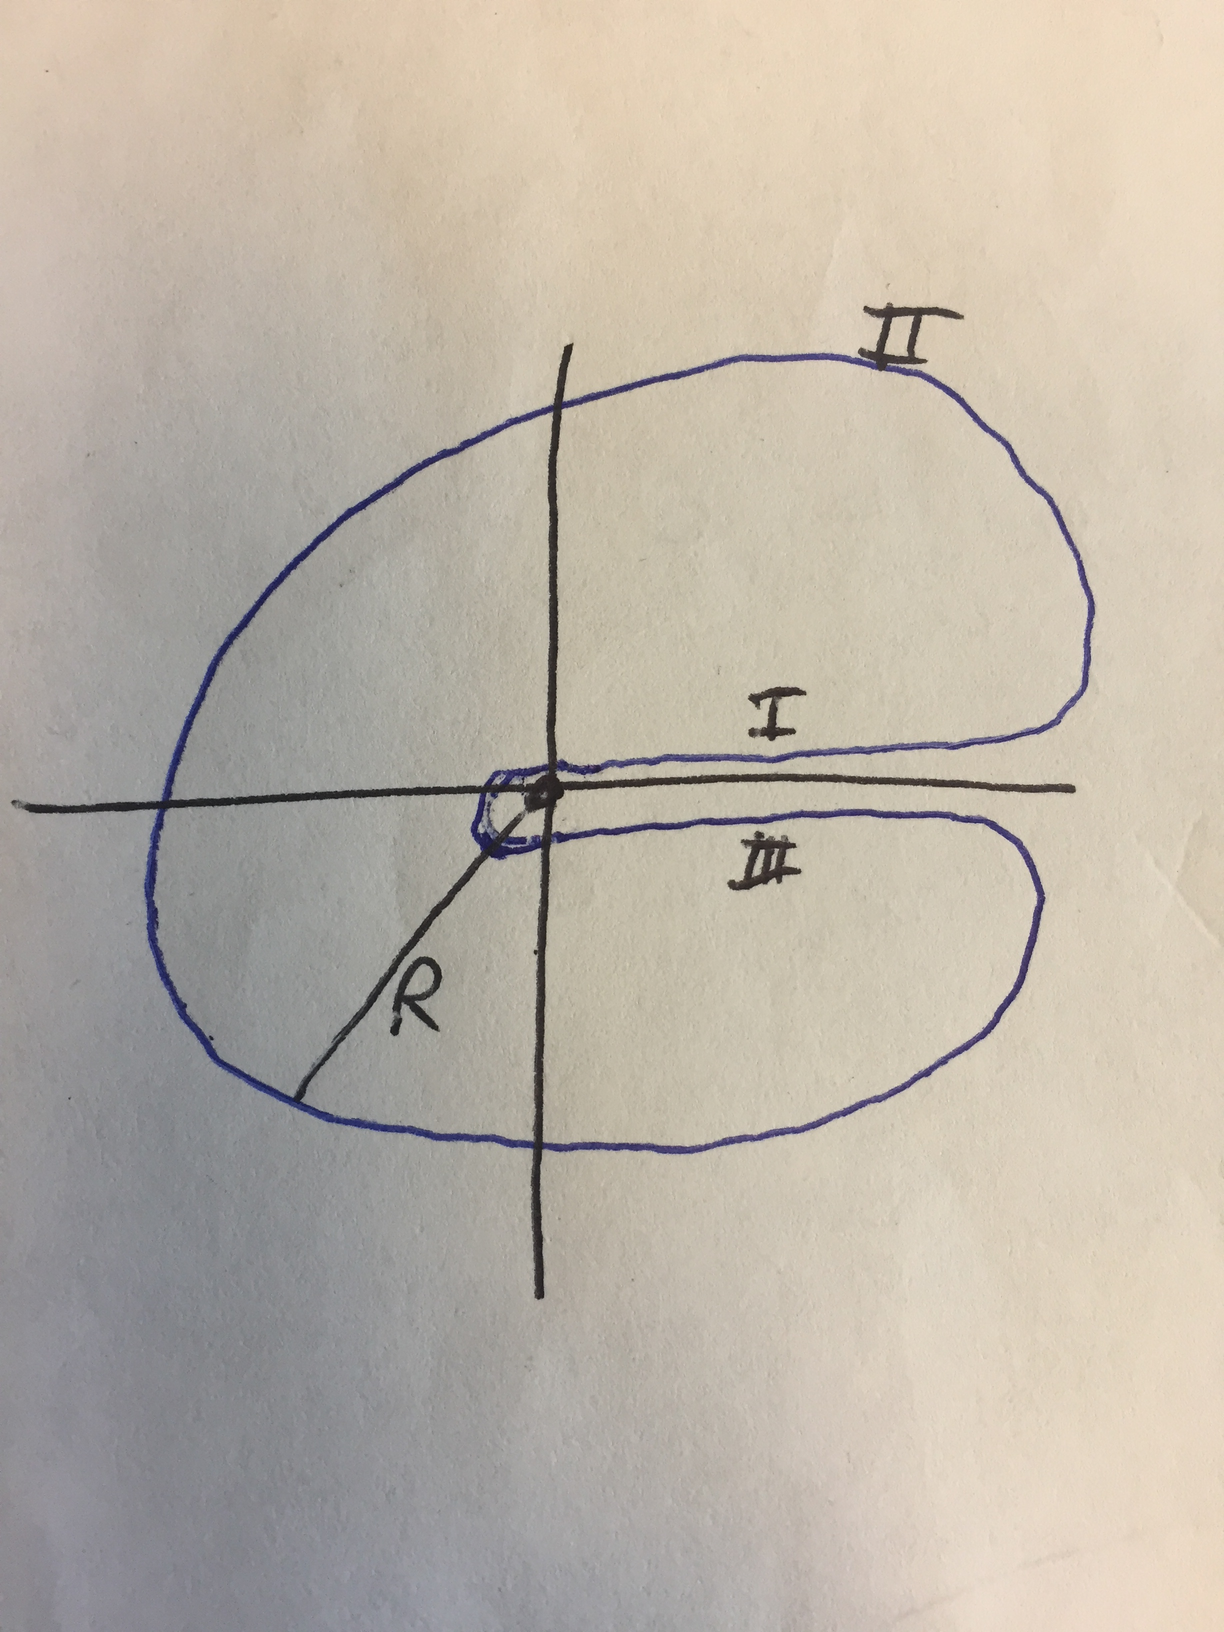
\includegraphics[scale=0.2]{Figures/log.png}
    \caption{Make a caption. I from 0-R, II circle, III R-0. Contour around natural log branching point at 0. ALSO REMEMBER TO PUT THE POLES IN (SAME AS LAST PROBLEM) 3 POLES -1, and the other 2. }
\end{figure}

%%%%%%%%%%%%%%%%%%%%%%%%%%%%%Need to do this math%%%%%%%%%%%%%%%%%%%%%%%%%%%%%%%%%%%%%%%%%%%%%%%%%%%%%%%%%%%%
With this contour you can do some math and you find the residue to be 
\be
\frac{4\pi^2i\sqrt{3}}{9}
\ee
%%%%%%%%%%%%%%%%%%%%%%%%%%%%%Need to do this math%%%%%%%%%%%%%%%%%%%%%%%%%%%%%%%%%%%%%%%%%%%%%%%%%%%%%%%%%%%%












\end{document}
